\documentclass[twoside]{book}

% Packages required by doxygen
\usepackage{fixltx2e}
\usepackage{calc}
\usepackage{doxygen}
\usepackage[export]{adjustbox} % also loads graphicx
\usepackage{graphicx}
\usepackage[utf8]{inputenc}
\usepackage{makeidx}
\usepackage{multicol}
\usepackage{multirow}
\PassOptionsToPackage{warn}{textcomp}
\usepackage{textcomp}
\usepackage[nointegrals]{wasysym}
\usepackage[table]{xcolor}

% Font selection
\usepackage[T1]{fontenc}
\usepackage[scaled=.90]{helvet}
\usepackage{courier}
\usepackage{amssymb}
\usepackage{sectsty}
\renewcommand{\familydefault}{\sfdefault}
\allsectionsfont{%
  \fontseries{bc}\selectfont%
  \color{darkgray}%
}
\renewcommand{\DoxyLabelFont}{%
  \fontseries{bc}\selectfont%
  \color{darkgray}%
}
\newcommand{\+}{\discretionary{\mbox{\scriptsize$\hookleftarrow$}}{}{}}

% Page & text layout
\usepackage{geometry}
\geometry{%
  a4paper,%
  top=2.5cm,%
  bottom=2.5cm,%
  left=2.5cm,%
  right=2.5cm%
}
\tolerance=750
\hfuzz=15pt
\hbadness=750
\setlength{\emergencystretch}{15pt}
\setlength{\parindent}{0cm}
\setlength{\parskip}{3ex plus 2ex minus 2ex}
\makeatletter
\renewcommand{\paragraph}{%
  \@startsection{paragraph}{4}{0ex}{-1.0ex}{1.0ex}{%
    \normalfont\normalsize\bfseries\SS@parafont%
  }%
}
\renewcommand{\subparagraph}{%
  \@startsection{subparagraph}{5}{0ex}{-1.0ex}{1.0ex}{%
    \normalfont\normalsize\bfseries\SS@subparafont%
  }%
}
\makeatother

% Headers & footers
\usepackage{fancyhdr}
\pagestyle{fancyplain}
\fancyhead[LE]{\fancyplain{}{\bfseries\thepage}}
\fancyhead[CE]{\fancyplain{}{}}
\fancyhead[RE]{\fancyplain{}{\bfseries\leftmark}}
\fancyhead[LO]{\fancyplain{}{\bfseries\rightmark}}
\fancyhead[CO]{\fancyplain{}{}}
\fancyhead[RO]{\fancyplain{}{\bfseries\thepage}}
\fancyfoot[LE]{\fancyplain{}{}}
\fancyfoot[CE]{\fancyplain{}{}}
\fancyfoot[RE]{\fancyplain{}{\bfseries\scriptsize Generated by Doxygen }}
\fancyfoot[LO]{\fancyplain{}{\bfseries\scriptsize Generated by Doxygen }}
\fancyfoot[CO]{\fancyplain{}{}}
\fancyfoot[RO]{\fancyplain{}{}}
\renewcommand{\footrulewidth}{0.4pt}
\renewcommand{\chaptermark}[1]{%
  \markboth{#1}{}%
}
\renewcommand{\sectionmark}[1]{%
  \markright{\thesection\ #1}%
}

% Indices & bibliography
\usepackage{natbib}
\usepackage[titles]{tocloft}
\setcounter{tocdepth}{3}
\setcounter{secnumdepth}{5}
\makeindex

% Hyperlinks (required, but should be loaded last)
\usepackage{ifpdf}
\ifpdf
  \usepackage[pdftex,pagebackref=true]{hyperref}
\else
  \usepackage[ps2pdf,pagebackref=true]{hyperref}
\fi
\hypersetup{%
  colorlinks=true,%
  linkcolor=blue,%
  citecolor=blue,%
  unicode%
}

% Custom commands
\newcommand{\clearemptydoublepage}{%
  \newpage{\pagestyle{empty}\cleardoublepage}%
}

\usepackage{caption}
\captionsetup{labelsep=space,justification=centering,font={bf},singlelinecheck=off,skip=4pt,position=top}

%===== C O N T E N T S =====

\begin{document}

% Titlepage & ToC
\hypersetup{pageanchor=false,
             bookmarksnumbered=true,
             pdfencoding=unicode
            }
\pagenumbering{roman}
\begin{titlepage}
\vspace*{7cm}
\begin{center}%
{\Large Scheduling simulation project for operating system \\[1ex]\large 1.\+0 }\\
\vspace*{1cm}
{\large Generated by Doxygen 1.8.11}\\
\end{center}
\end{titlepage}
\clearemptydoublepage
\tableofcontents
\clearemptydoublepage
\pagenumbering{arabic}
\hypersetup{pageanchor=true}

%--- Begin generated contents ---
\chapter{File Index}
\section{File List}
Here is a list of all files with brief descriptions\+:\begin{DoxyCompactList}
\item\contentsline{section}{\hyperlink{main_8c}{main.\+c} }{\pageref{main_8c}}{}
\end{DoxyCompactList}

\chapter{File Documentation}
\hypertarget{main_8c}{}\section{main.\+c File Reference}
\label{main_8c}\index{main.\+c@{main.\+c}}
{\ttfamily \#include $<$stdio.\+h$>$}\\*
{\ttfamily \#include $<$string.\+h$>$}\\*
Include dependency graph for main.\+c\+:
\nopagebreak
\begin{figure}[H]
\begin{center}
\leavevmode
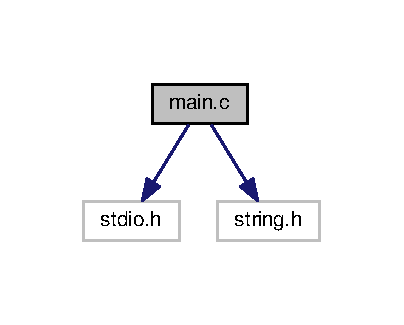
\includegraphics[width=194pt]{main_8c__incl}
\end{center}
\end{figure}
\subsection*{Macros}
\begin{DoxyCompactItemize}
\item 
\#define \hyperlink{main_8c_af5af0676a4c31aa406bbb958e78ce48a}{N\+B\+P\+R\+O\+C\+E\+S\+S\+M\+AX}~1000
\end{DoxyCompactItemize}
\subsection*{Functions}
\begin{DoxyCompactItemize}
\item 
int \hyperlink{main_8c_a17711d4315788fc64017dbdc037e3cc5}{fifo} (int n, int bt\mbox{[}$\,$\mbox{]})
\item 
int \hyperlink{main_8c_a020dc3c37c12bc10e0b14c9f27d07b1d}{sjf} (int n, int bt\mbox{[}$\,$\mbox{]})
\item 
int \hyperlink{main_8c_a19b487367aa01ea15f3235f3ac6db074}{sjrf} (int n, int bt\mbox{[}n\mbox{]}, int pr\mbox{[}n\mbox{]})
\item 
int \hyperlink{main_8c_a91b876a340d90758b01762b02028bca5}{rr} (int n, int bt\mbox{[}n\mbox{]}, int at\mbox{[}n\mbox{]}, int time\+\_\+quantum)
\item 
int \hyperlink{main_8c_aa9ef50688f151d720461502ef1ff9c3b}{reading\+\_\+from\+\_\+file} (int $\ast$n, int bt\mbox{[}$\,$\mbox{]}, int priorities\mbox{[}$\,$\mbox{]}, int arrival\+\_\+time\mbox{[}$\,$\mbox{]}, int $\ast$quantum\+\_\+time, int $\ast$chosen\+\_\+algo)
\item 
int \hyperlink{main_8c_ae66f6b31b5ad750f1fe042a706a4e3d4}{main} ()
\end{DoxyCompactItemize}


\subsection{Macro Definition Documentation}
\index{main.\+c@{main.\+c}!N\+B\+P\+R\+O\+C\+E\+S\+S\+M\+AX@{N\+B\+P\+R\+O\+C\+E\+S\+S\+M\+AX}}
\index{N\+B\+P\+R\+O\+C\+E\+S\+S\+M\+AX@{N\+B\+P\+R\+O\+C\+E\+S\+S\+M\+AX}!main.\+c@{main.\+c}}
\subsubsection[{\texorpdfstring{N\+B\+P\+R\+O\+C\+E\+S\+S\+M\+AX}{NBPROCESSMAX}}]{\setlength{\rightskip}{0pt plus 5cm}\#define N\+B\+P\+R\+O\+C\+E\+S\+S\+M\+AX~1000}\hypertarget{main_8c_af5af0676a4c31aa406bbb958e78ce48a}{}\label{main_8c_af5af0676a4c31aa406bbb958e78ce48a}


\subsection{Function Documentation}
\index{main.\+c@{main.\+c}!fifo@{fifo}}
\index{fifo@{fifo}!main.\+c@{main.\+c}}
\subsubsection[{\texorpdfstring{fifo(int n, int bt[])}{fifo(int n, int bt[])}}]{\setlength{\rightskip}{0pt plus 5cm}int fifo (
\begin{DoxyParamCaption}
\item[{int}]{n, }
\item[{int}]{bt\mbox{[}$\,$\mbox{]}}
\end{DoxyParamCaption}
)}\hypertarget{main_8c_a17711d4315788fc64017dbdc037e3cc5}{}\label{main_8c_a17711d4315788fc64017dbdc037e3cc5}

\begin{DoxyCode}
7                             \{
8       \textcolor{comment}{//array of waiting time}
9       \textcolor{keywordtype}{int} wt[n],
10       \textcolor{comment}{//array of turnaround time }
11       tat[n],
12       \textcolor{comment}{//average waiting time initialised with 0 at the first time}
13       avwt=0,
14      \textcolor{comment}{//average turnaround time }
15       avtat=0,
16       i,j;
17      \textcolor{comment}{//waiting time for first process is 0}
18        wt[0] = 0;   
19     
20         \textcolor{comment}{//to calculate waiting time}
21         \textcolor{keywordflow}{for}(i=1;i<n;i++)
22         \{
23             wt[i]=0;
24             \textcolor{keywordflow}{for}(j=0;j<i;j++)
25                 wt[i]+=bt[j];
26         \}
27 
28      printf(\textcolor{stringliteral}{"\(\backslash\)nProcess\(\backslash\)t\(\backslash\)tBurst Time\(\backslash\)tWaiting Time\(\backslash\)tTurnaround Time"});
29 
30        \textcolor{comment}{// to calculate turnaround time}
31         \textcolor{keywordflow}{for}(i=0;i<n;i++)
32         \{
33             tat[i]=bt[i]+wt[i];
34             avwt+=wt[i];
35             avtat+=tat[i];
36         \textcolor{comment}{//display the result}
37             printf(\textcolor{stringliteral}{"\(\backslash\)nP[%d]\(\backslash\)t\(\backslash\)t%d\(\backslash\)t\(\backslash\)t%d\(\backslash\)t\(\backslash\)t%d"},i+1,bt[i],wt[i],tat[i]); 
38         \}
39     
40         avwt/=i;
41         avtat/=i;
42         \textcolor{comment}{//display Average Waiting Time}
43         printf(\textcolor{stringliteral}{"\(\backslash\)n\(\backslash\)nAverage Waiting Time:%d"},avwt);
44         \textcolor{comment}{//display Average Turnaround Time}
45         printf(\textcolor{stringliteral}{"\(\backslash\)nAverage Turnaround Time:%d \(\backslash\)n"},avtat);
46     
47         \textcolor{keywordflow}{return} 0;
48 \}
\end{DoxyCode}
\index{main.\+c@{main.\+c}!main@{main}}
\index{main@{main}!main.\+c@{main.\+c}}
\subsubsection[{\texorpdfstring{main()}{main()}}]{\setlength{\rightskip}{0pt plus 5cm}int main (
\begin{DoxyParamCaption}
{}
\end{DoxyParamCaption}
)}\hypertarget{main_8c_ae66f6b31b5ad750f1fe042a706a4e3d4}{}\label{main_8c_ae66f6b31b5ad750f1fe042a706a4e3d4}

\begin{DoxyCode}
401             \{
402      \textcolor{keywordtype}{int} n,i,j,f;
403      \textcolor{keywordtype}{int} bt[\hyperlink{main_8c_af5af0676a4c31aa406bbb958e78ce48a}{NBPROCESSMAX}];
404      \textcolor{keywordtype}{int} priorities[\hyperlink{main_8c_af5af0676a4c31aa406bbb958e78ce48a}{NBPROCESSMAX}];
405      \textcolor{keywordtype}{int} arrival\_time[\hyperlink{main_8c_af5af0676a4c31aa406bbb958e78ce48a}{NBPROCESSMAX}];
406      \textcolor{keywordtype}{int} quantum\_time;
407      \textcolor{keywordtype}{int} chosen\_algo;
408 
409 \textcolor{keywordflow}{do}\{
410      printf(\textcolor{stringliteral}{"\(\backslash\)nEnter 1 to read input from the file 'input\_file.txt'. \(\backslash\)nEnter 2 for manual input. \(\backslash\)nEnter 3
       to exit\(\backslash\)n"});
411      scanf(\textcolor{stringliteral}{"%d"},&f);
412         \textcolor{keywordflow}{if} (f == 1) \{
413              \hyperlink{main_8c_aa9ef50688f151d720461502ef1ff9c3b}{reading\_from\_file}(&n, bt, priorities, arrival\_time, &quantum\_time, &
      chosen\_algo);
414         \}
415 
416         \textcolor{keywordflow}{else} \textcolor{keywordflow}{if} (f == 2) \{
417              printf(\textcolor{stringliteral}{"Enter Total Number of Process:"});
418              scanf(\textcolor{stringliteral}{"%d"},&n);
419 
420              printf(\textcolor{stringliteral}{"\(\backslash\)nEnter Process Burst Time\(\backslash\)n"});
421              \textcolor{keywordflow}{for}(i=0;i<n;i++)
422              \{
423                  printf(\textcolor{stringliteral}{"P[%d]:"},i+1);
424                  scanf(\textcolor{stringliteral}{"%d"},&bt[i]);
425              \}
426 
427              printf(\textcolor{stringliteral}{"Chose your algorithm...Enter:\(\backslash\)n1 for FIFO.\(\backslash\)n2 for SJF.\(\backslash\)n3 for SJRF.\(\backslash\)n4 for RR\(\backslash\)n"});
428              scanf(\textcolor{stringliteral}{"%d"}, &chosen\_algo);
429 
430 
431              \textcolor{keywordflow}{if} (chosen\_algo == 3) \{
432                   printf(\textcolor{stringliteral}{"\(\backslash\)nEnter Priorities times\(\backslash\)n"});
433                   \textcolor{keywordflow}{for}(i=0;i<n;i++)
434                   \{
435                       printf(\textcolor{stringliteral}{"P[%d]:"},i+1);
436                       scanf(\textcolor{stringliteral}{"%d"},&priorities[i]);
437                   \}
438              \}
439 
440              \textcolor{keywordflow}{if} (chosen\_algo == 4) \{
441                   printf(\textcolor{stringliteral}{"\(\backslash\)nEnter Arrivals Times\(\backslash\)n"});
442                   \textcolor{keywordflow}{for}(i=0;i<n;i++)
443                   \{
444                       printf(\textcolor{stringliteral}{"P[%d]:"},i+1);
445                       scanf(\textcolor{stringliteral}{"%d"},&arrival\_time[i]);
446                   \}
447                   printf(\textcolor{stringliteral}{"\(\backslash\)nEnter Quantum Time\(\backslash\)n"});
448                   scanf(\textcolor{stringliteral}{"%d"},&quantum\_time);
449              \}
450         \}
451     \textcolor{keywordflow}{else} \{
452         \textcolor{keywordflow}{if}(f == 3) \{
453             \textcolor{keywordflow}{break};
454         \}
455     \}
456 
457 
458         \textcolor{comment}{/* Menu displaying all the chosen configurations */}
459 
460         printf(\textcolor{stringliteral}{".....................................................\(\backslash\)n"});
461         printf(\textcolor{stringliteral}{"...............Choosed configurations................\(\backslash\)n"});
462         printf(\textcolor{stringliteral}{".....................................................\(\backslash\)n \(\backslash\)n"});
463 
464         \textcolor{keywordflow}{if} (chosen\_algo == 1) \{
465              printf(\textcolor{stringliteral}{"Chosen Algorithm.................. FIFO. \(\backslash\)n"}, n);
466              printf(\textcolor{stringliteral}{"Number of processes.................. %d \(\backslash\)n"}, n);
467 
468         \}
469 
470         \textcolor{keywordflow}{if} (chosen\_algo == 2) \{
471             printf(\textcolor{stringliteral}{"Chosen Algorithm.................. SFJ. \(\backslash\)n"}, n);
472             printf(\textcolor{stringliteral}{"Number of processes.................. %d \(\backslash\)n"}, n);
473         \}
474 
475         \textcolor{keywordflow}{if} (chosen\_algo == 3) \{
476              printf(\textcolor{stringliteral}{"Chosen Algorithm.................. SJRF. \(\backslash\)n"}, n);
477              printf(\textcolor{stringliteral}{"Number of processes.................. %d \(\backslash\)n"}, n);
478 
479         \}
480 
481         \textcolor{keywordflow}{if} (chosen\_algo == 4) \{
482             printf(\textcolor{stringliteral}{"Chosen Algorithm.................. RR \(\backslash\)n"}, n);
483             printf(\textcolor{stringliteral}{"Quantum Time.................. %d \(\backslash\)n"}, quantum\_time);
484         \}
485 
486 
487 
488 
489         \textcolor{comment}{/* Running the algo */}
490 
491         \textcolor{keywordflow}{if} (chosen\_algo == 1) \{
492              \hyperlink{main_8c_a17711d4315788fc64017dbdc037e3cc5}{fifo}(n, bt);
493         \}
494 
495         \textcolor{keywordflow}{if} (chosen\_algo == 2) \{
496              \hyperlink{main_8c_a020dc3c37c12bc10e0b14c9f27d07b1d}{sjf}(n, bt);
497         \}
498 
499         \textcolor{keywordflow}{if} (chosen\_algo == 3 ) \{
500              \hyperlink{main_8c_a19b487367aa01ea15f3235f3ac6db074}{sjrf}(n, bt, priorities);
501         \}
502 
503         \textcolor{keywordflow}{if} (chosen\_algo == 4) \{
504              \hyperlink{main_8c_a91b876a340d90758b01762b02028bca5}{rr}(n, bt, arrival\_time, quantum\_time);
505         \}
506 \}\textcolor{keywordflow}{while}(f!=3);
507 
508 \}
\end{DoxyCode}
\index{main.\+c@{main.\+c}!reading\+\_\+from\+\_\+file@{reading\+\_\+from\+\_\+file}}
\index{reading\+\_\+from\+\_\+file@{reading\+\_\+from\+\_\+file}!main.\+c@{main.\+c}}
\subsubsection[{\texorpdfstring{reading\+\_\+from\+\_\+file(int $\ast$n, int bt[], int priorities[], int arrival\+\_\+time[], int $\ast$quantum\+\_\+time, int $\ast$chosen\+\_\+algo)}{reading_from_file(int *n, int bt[], int priorities[], int arrival_time[], int *quantum_time, int *chosen_algo)}}]{\setlength{\rightskip}{0pt plus 5cm}int reading\+\_\+from\+\_\+file (
\begin{DoxyParamCaption}
\item[{int $\ast$}]{n, }
\item[{int}]{bt\mbox{[}$\,$\mbox{]}, }
\item[{int}]{priorities\mbox{[}$\,$\mbox{]}, }
\item[{int}]{arrival\+\_\+time\mbox{[}$\,$\mbox{]}, }
\item[{int $\ast$}]{quantum\+\_\+time, }
\item[{int $\ast$}]{chosen\+\_\+algo}
\end{DoxyParamCaption}
)}\hypertarget{main_8c_aa9ef50688f151d720461502ef1ff9c3b}{}\label{main_8c_aa9ef50688f151d720461502ef1ff9c3b}

\begin{DoxyCode}
269                                                                                                            
               \{
270      \textcolor{keywordtype}{int} line\_counter = 1;
271      FILE* fichier = NULL;
272     \textcolor{keywordtype}{char} c;
273     fichier = fopen(\textcolor{stringliteral}{"input\_file.txt"}, \textcolor{stringliteral}{"r"});
274     \textcolor{keywordtype}{char} line\_string[1000];
275     \textcolor{keywordtype}{char} number\_string[5];
276     \textcolor{keywordtype}{int} i, j, k, n\_aux, nb\_proc;
277 
278     \textcolor{keywordflow}{if}(fichier != NULL)\{
279          \textcolor{keywordflow}{if} (line\_counter == 1) \{
280               fgets(number\_string, 1000, fichier);
281               nb\_proc = atoi(number\_string);
282               *n = nb\_proc;
283               line\_counter++;
284               strcpy(number\_string, \textcolor{stringliteral}{""});
285          \}
286 
287          \textcolor{keywordflow}{if} (line\_counter == 2) \{
288               fgets(line\_string, 1000, fichier);
289               i = 0;
290               j = 0;
291               k = 0;
292               c = line\_string[0];
293               \textcolor{keywordflow}{while} (c != \textcolor{charliteral}{'\(\backslash\)n'}) \{
294                    c = line\_string[i];
295                    \textcolor{keywordflow}{if} (c != \textcolor{charliteral}{' '} && c != \textcolor{charliteral}{'\(\backslash\)n'}) \{
296                         number\_string[j] = c;
297                         j++;
298                    \}
299                    \textcolor{keywordflow}{else} \{
300                         j = 0;
301                         n\_aux = atoi(number\_string);
302                         bt[k] = n\_aux;
303                         k++;
304                         strcpy(number\_string, \textcolor{stringliteral}{""});
305                         \textcolor{comment}{//printf("%d ", n\_aux);}
306                    \}
307                    i++;
308               \}
309               line\_counter++;
310 
311          \}
312 
313          \textcolor{keywordflow}{if} (line\_counter == 3) \{
314               fgets(number\_string, 5, fichier);
315               *chosen\_algo = atoi(number\_string);
316               \textcolor{comment}{/* FIFO */}
317               \textcolor{keywordflow}{if} (n\_aux == 1) \{
318                    fclose(fichier);
319                    \textcolor{keywordflow}{return} 0;
320               \}
321 
322               \textcolor{comment}{/* SFJ */}
323               \textcolor{keywordflow}{if} (n\_aux == 2) \{
324                    fclose(fichier);
325                    \textcolor{keywordflow}{return} 0;
326               \}
327 
328               line\_counter++;
329               strcpy(number\_string, \textcolor{stringliteral}{""});
330          \}
331 
332          \textcolor{keywordflow}{if} (line\_counter == 4) \{
333               \textcolor{keywordflow}{if} (*chosen\_algo == 3) \{
334                    strcpy(line\_string, \textcolor{stringliteral}{""});
335                    fgets(line\_string, 1000, fichier);
336                    i = 0;
337                    j = 0;
338                    k = 0;
339                    c = line\_string[0];
340                    \textcolor{keywordflow}{while} (c != \textcolor{charliteral}{'\(\backslash\)n'}) \{
341                         c = line\_string[i];
342                         \textcolor{keywordflow}{if} (c != \textcolor{charliteral}{' '} && c != \textcolor{charliteral}{'\(\backslash\)n'}) \{
343                              number\_string[j] = c;
344                              j++;
345                         \}
346                         \textcolor{keywordflow}{else} \{
347                              j = 0;
348                              n\_aux = atoi(number\_string);
349                              priorities[k] = n\_aux;
350                              k++;
351                              strcpy(number\_string, \textcolor{stringliteral}{""});
352                              \textcolor{comment}{//printf("%d ", n\_aux);}
353                         \}
354                         i++;
355                    \}
356 
357                    fclose(fichier);
358                    \textcolor{keywordflow}{return} 0;
359               \}
360 
361               \textcolor{keywordflow}{else} \textcolor{keywordflow}{if} (*chosen\_algo == 4) \{
362                    strcpy(line\_string, \textcolor{stringliteral}{""});
363                    fgets(line\_string, 1000, fichier);
364                    i = 0;
365                    j = 0;
366                    k = 0;
367                    c = line\_string[0];
368                    \textcolor{keywordflow}{while} (c != \textcolor{charliteral}{'\(\backslash\)n'}) \{
369                         c = line\_string[i];
370                         \textcolor{keywordflow}{if} (c != \textcolor{charliteral}{' '} && c != \textcolor{charliteral}{'\(\backslash\)n'}) \{
371                              number\_string[j] = c;
372                              j++;
373                         \}
374                         \textcolor{keywordflow}{else} \{
375                              j = 0;
376                              n\_aux = atoi(number\_string);
377                              arrival\_time[k] = n\_aux;
378                              k++;
379                              strcpy(number\_string, \textcolor{stringliteral}{""});
380                              \textcolor{comment}{//printf("%d ", n\_aux);}
381                         \}
382                         i++;
383                    \}
384               \}
385              line\_counter++;
386          \}
387 
388          \textcolor{keywordflow}{if} (line\_counter == 5) \{
389               strcpy(number\_string, \textcolor{stringliteral}{""});
390               fgets(number\_string, 5, fichier);
391               *quantum\_time = atoi(number\_string);
392               fclose(fichier);
393               line\_counter = 0;
394               strcpy(number\_string, \textcolor{stringliteral}{""});
395               \textcolor{keywordflow}{return} 0;
396          \}
397     \}
398 \}
\end{DoxyCode}
\index{main.\+c@{main.\+c}!rr@{rr}}
\index{rr@{rr}!main.\+c@{main.\+c}}
\subsubsection[{\texorpdfstring{rr(int n, int bt[n], int at[n], int time\+\_\+quantum)}{rr(int n, int bt[n], int at[n], int time_quantum)}}]{\setlength{\rightskip}{0pt plus 5cm}int rr (
\begin{DoxyParamCaption}
\item[{int}]{n, }
\item[{int}]{bt\mbox{[}n\mbox{]}, }
\item[{int}]{at\mbox{[}n\mbox{]}, }
\item[{int}]{time\+\_\+quantum}
\end{DoxyParamCaption}
)}\hypertarget{main_8c_a91b876a340d90758b01762b02028bca5}{}\label{main_8c_a91b876a340d90758b01762b02028bca5}

\begin{DoxyCode}
179                                                        \{
180      \textcolor{keywordtype}{int} queue[1000];
181      \textcolor{keywordtype}{int} i,j,k,y,total = 0, x, finish\_flag = 0, current\_process, flag\_inQueue;
182         \textcolor{keywordtype}{int} wait\_time, turnaround\_time = 0, 
183     \textcolor{comment}{//temp is the remaining time for each process}
184     temp[n]; 
185         \textcolor{keywordtype}{float} total\_wait\_time = 0, total\_turnaround\_time = 0;
186     \textcolor{comment}{//countdown to be sure all process are finished}
187         x = n; 
188           \textcolor{keywordflow}{for}(j = 0; j < n; j++) \{
189              \textcolor{comment}{//initial remaining time is the burst time}
190                      temp[j] = bt[j]; 
191          \}
192 
193           printf(\textcolor{stringliteral}{"\(\backslash\)nProcess\(\backslash\)t\(\backslash\)tBurst Time\(\backslash\)tArrival Time\(\backslash\)tWaiting Time\(\backslash\)tTurnaround Time"});
194       \textcolor{comment}{//total time}
195           total = 0; 
196           \textcolor{comment}{/* the first process to enter in the queue is the first process, i keeps track of the actual
       position of the queue*/}
197           i = 0;
198       \textcolor{comment}{/* k keeps track of the last position */}
199           k = 0; 
200           queue[i] = 1;
201 
202           \textcolor{keywordflow}{while}(x != 0)
203         \{
204                current\_process = queue[i];
205 
206                \textcolor{comment}{/* if the remaining time is exactly the quantum time */}
207                 \textcolor{keywordflow}{if}(temp[current\_process-1] <= time\_quantum && temp[current\_process-1] > 0)
208                 \{
209                     total = total + temp[current\_process-1];
210                 \textcolor{comment}{//then the remaining time go to 0}
211                     temp[current\_process-1] = 0; 
212                 \}
213                 \textcolor{keywordflow}{else} \textcolor{keywordflow}{if}(temp[current\_process-1] > 0)
214                 \{
215                     temp[current\_process-1] = temp[current\_process-1] - time\_quantum;
216                     total = total + time\_quantum;
217                 \}
218                \textcolor{comment}{/*If the process has ended */}
219                 \textcolor{keywordflow}{if}(temp[current\_process-1] == 0)
220                 \{
221                 x--;
222                     turnaround\_time = total - at[current\_process-1];
223                     wait\_time = turnaround\_time - bt[current\_process-1];
224                 printf(\textcolor{stringliteral}{"\(\backslash\)nP[%d]\(\backslash\)t\(\backslash\)t%d\(\backslash\)t\(\backslash\)t%d\(\backslash\)t\(\backslash\)t%d\(\backslash\)t\(\backslash\)t%d"}, current\_process, bt[current\_process-1], at[
      current\_process-1], wait\_time, turnaround\_time);
225 
226                     total\_wait\_time = total\_wait\_time + wait\_time;
227                          total\_turnaround\_time = total\_turnaround\_time + turnaround\_time;
228 
229                 \}
230 
231                \textcolor{comment}{/* For every other process, sees if they reached their arrival time */}
232                \textcolor{keywordflow}{for}(j = 0; j < n; j++) \{
233                     \textcolor{comment}{/* Insert the process in the queue if needed*/}
234                     \textcolor{keywordflow}{if} (at[j] <= total && temp[j] != 0 && j != current\_process-1) \{
235                          flag\_inQueue = 0;
236                          \textcolor{comment}{/* Verifies first if the process is already in the queue  */}
237                          \textcolor{keywordflow}{for} (y=i; y <= k; y++) \{
238                               \textcolor{keywordflow}{if} (queue[y] == j+1) \{
239                                    flag\_inQueue = 1;
240                                    \textcolor{keywordflow}{break};
241                               \}
242                          \}
243                          \textcolor{comment}{/* if its not, insert in the queue */}
244                          \textcolor{keywordflow}{if} (flag\_inQueue == 0) \{
245                               queue[k+1] = j+1;
246                               k++;
247                          \}
248 
249                     \}
250                \}
251 
252                \textcolor{comment}{/*If the current process is not finished yet, put it in the queue*/}
253                \textcolor{keywordflow}{if} (temp[current\_process-1] != 0) \{
254                     queue[k+1] = current\_process;
255                     k++;
256                \}
257 
258                i++;
259         \}
260 
261         \textcolor{keywordtype}{float} average\_wait\_time = total\_wait\_time * 1.0 / n;
262         \textcolor{keywordtype}{float} average\_turnaround\_time = total\_turnaround\_time * 1.0 / n;
263         printf(\textcolor{stringliteral}{"\(\backslash\)n\(\backslash\)nAverage Waiting Time:\(\backslash\)t%f"}, average\_wait\_time);
264         printf(\textcolor{stringliteral}{"\(\backslash\)nAvg Turnaround Time:\(\backslash\)t%f\(\backslash\)n"}, average\_turnaround\_time);
265         \textcolor{keywordflow}{return} 0;
266 
267 \}
\end{DoxyCode}
\index{main.\+c@{main.\+c}!sjf@{sjf}}
\index{sjf@{sjf}!main.\+c@{main.\+c}}
\subsubsection[{\texorpdfstring{sjf(int n, int bt[])}{sjf(int n, int bt[])}}]{\setlength{\rightskip}{0pt plus 5cm}int sjf (
\begin{DoxyParamCaption}
\item[{int}]{n, }
\item[{int}]{bt\mbox{[}$\,$\mbox{]}}
\end{DoxyParamCaption}
)}\hypertarget{main_8c_a020dc3c37c12bc10e0b14c9f27d07b1d}{}\label{main_8c_a020dc3c37c12bc10e0b14c9f27d07b1d}

\begin{DoxyCode}
51                           \{
52      \textcolor{keywordtype}{int} p[n],
53      wt[n], tat[n],
54      i, j, total=0, pos, temp;
55      \textcolor{keywordtype}{float} avg\_wt,avg\_tat;
56     
57         \textcolor{keywordflow}{for}(i=0;i<n;i++) \{
58         \textcolor{comment}{//array contains number of process}
59             p[i]=i+1;           
60         \}
61         \textcolor{comment}{//sorting burst time in ascending order using selection sort}
62         \textcolor{keywordflow}{for}(i=0;i<n;i++) \{
63             pos=i;
64             \textcolor{keywordflow}{for}(j=i+1;j<n;j++) \{
65                 \textcolor{keywordflow}{if}(bt[j]<bt[pos])
66                     pos=j;
67             \}
68     
69             temp=bt[i];
70             bt[i]=bt[pos];
71             bt[pos]=temp;
72     
73             temp=p[i];
74             p[i]=p[pos];
75             p[pos]=temp;
76         \}
77         
78         \textcolor{comment}{//waiting time for first process will be zero}
79         wt[0]=0;           
80     
81         \textcolor{comment}{//to calculate waiting time}
82         \textcolor{keywordflow}{for}(i=1;i<n;i++)
83         \{
84             wt[i]=0;
85             \textcolor{keywordflow}{for}(j=0;j<i;j++)
86                 wt[i]+=bt[j];
87     
88             total+=wt[i];
89         \}
90         
91         \textcolor{comment}{//average waiting time}
92         avg\_wt=(float)total/n;      
93         total=0;
94     
95         printf(\textcolor{stringliteral}{"\(\backslash\)nProcess\(\backslash\)t    Burst Time    \(\backslash\)tWaiting Time\(\backslash\)tTurnaround Time"});
96         \textcolor{keywordflow}{for}(i=0;i<n;i++)
97         \{   
98         \textcolor{comment}{//to calculate turnaround time}
99            tat[i]=bt[i]+wt[i];     
100            total+=tat[i];
101            printf(\textcolor{stringliteral}{"\(\backslash\)nP[%d]\(\backslash\)t\(\backslash\)t  %d\(\backslash\)t\(\backslash\)t    %d\(\backslash\)t\(\backslash\)t\(\backslash\)t%d"},p[i],bt[i],wt[i],tat[i]);
102        \}
103    
104        avg\_tat=(float)total/n;    
105        printf(\textcolor{stringliteral}{"\(\backslash\)n\(\backslash\)nAverage Waiting Time=%.2f"}, avg\_wt);
106        printf(\textcolor{stringliteral}{"\(\backslash\)nAverage Turnaround Time=%.2f\(\backslash\)n"}, avg\_tat);
107    
108 \}
\end{DoxyCode}
\index{main.\+c@{main.\+c}!sjrf@{sjrf}}
\index{sjrf@{sjrf}!main.\+c@{main.\+c}}
\subsubsection[{\texorpdfstring{sjrf(int n, int bt[n], int pr[n])}{sjrf(int n, int bt[n], int pr[n])}}]{\setlength{\rightskip}{0pt plus 5cm}int sjrf (
\begin{DoxyParamCaption}
\item[{int}]{n, }
\item[{int}]{bt\mbox{[}n\mbox{]}, }
\item[{int}]{pr\mbox{[}n\mbox{]}}
\end{DoxyParamCaption}
)}\hypertarget{main_8c_a19b487367aa01ea15f3235f3ac6db074}{}\label{main_8c_a19b487367aa01ea15f3235f3ac6db074}

\begin{DoxyCode}
112                                        \{
113      \textcolor{keywordtype}{int} wt[n],tat[n],p[n], i,j,total=0,pos,temp;
114      \textcolor{keywordtype}{float} avg\_wt = 0, avg\_tat = 0;
115 
116      \textcolor{keywordflow}{for}(i=0;i<n;i++) \{
117      \textcolor{comment}{//contains process number}
118          p[i]=i+1;           
119      \}
120 
121      \textcolor{comment}{//sorting burst time, priority and process number in ascending order using selection sort}
122      \textcolor{keywordflow}{for}(i=0;i<n;i++)
123      \{
124          pos=i;
125          \textcolor{keywordflow}{for}(j=i+1;j<n;j++)
126          \{
127             \textcolor{keywordflow}{if}(pr[j]<pr[pos])
128                  pos=j;
129          \}
130 
131          temp=pr[i];
132          pr[i]=pr[pos];
133          pr[pos]=temp;
134 
135          temp=bt[i];
136          bt[i]=bt[pos];
137          bt[pos]=temp;
138 
139          temp=p[i];
140          p[i]=p[pos];
141          p[pos]=temp;
142      \}
143      \textcolor{comment}{//waiting time for first process is zero}
144      wt[0]=0;    
145 
146      \textcolor{comment}{//calculate waiting time}
147      \textcolor{keywordflow}{for}(i=1;i<n;i++)
148      \{
149          wt[i]=0;
150          \textcolor{keywordflow}{for}(j=0;j<i;j++)
151             wt[i]+=bt[j];
152 
153          total+=wt[i];
154      \}
155      
156      \textcolor{comment}{//to calculate average waiting time}
157      avg\_wt=total/n;      
158      total=0;
159 
160      printf(\textcolor{stringliteral}{"\(\backslash\)nProcess\(\backslash\)t\(\backslash\)tBurst Time\(\backslash\)tPriority Time\(\backslash\)tWaiting Time\(\backslash\)tTurnaround Time"});
161      \textcolor{keywordflow}{for}(i=0;i<n;i++)
162      \{
163      \textcolor{comment}{//calculate turnaround time}
164          tat[i]=bt[i]+wt[i];     
165          total+=tat[i];
166          printf(\textcolor{stringliteral}{"\(\backslash\)nP[%d]\(\backslash\)t\(\backslash\)t%d\(\backslash\)t\(\backslash\)t%d\(\backslash\)t\(\backslash\)t%d\(\backslash\)t\(\backslash\)t%d"},p[i],bt[i],pr[i],wt[i],tat[i]);
167      \}
168 
169      \textcolor{comment}{//average turnaround time}
170      avg\_tat=total/n;    
171      printf(\textcolor{stringliteral}{"\(\backslash\)n\(\backslash\)nAverage Waiting Time=%.2f"},avg\_wt);
172      printf(\textcolor{stringliteral}{"\(\backslash\)nAverage Turnaround Time=%.2f\(\backslash\)n"},avg\_tat);
173 
174      \textcolor{keywordflow}{return} 0;
175 
176 \}
\end{DoxyCode}

%--- End generated contents ---

% Index
\backmatter
\newpage
\phantomsection
\clearemptydoublepage
\addcontentsline{toc}{chapter}{Index}
\printindex

\end{document}
